% Asset ID: AS1ExponentialsAndLogarithmsTikZ-003
% Asset type: TikZ diagram
% Suggested file path: tikz/AS1ExponentialsAndLogarithmsTikZ-003.tex
% Unit code: AS1
% Topic code: AS1-EXPLOG
% Topic name: Exponentials and logarithms
% Related lesson section: Core Theory 11; Visual Asset Integration
% Source: CCEA AS1-EXPLOG inverse function boundary; Chapter 14 logarithm evidence
% Purpose: Show y = e^x and y = ln x as inverse functions reflected in y = x.
\documentclass[tikz,border=8pt]{standalone}
\usepackage{amsmath}
\usepackage{pgfplots}
\pgfplotsset{compat=1.18}
\begin{document}
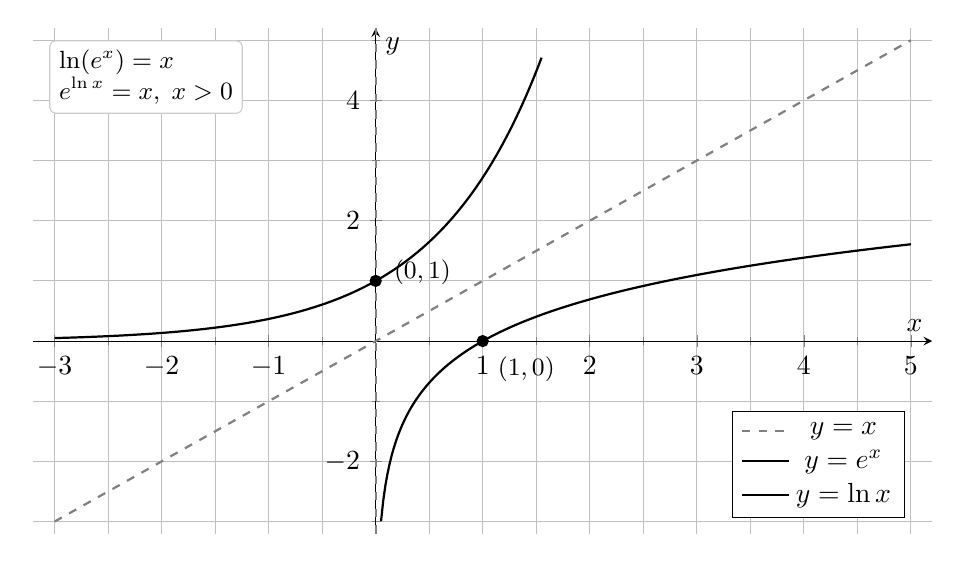
\begin{tikzpicture}
\begin{axis}[width=13cm,height=8cm,axis lines=middle,xmin=-3.2,xmax=5.2,ymin=-3.2,ymax=5.2,xlabel={$x$},ylabel={$y$},grid=both,minor tick num=1,samples=250,legend pos=south east]
\addplot[dashed,thick,gray,domain=-3:5]{x};\addlegendentry{$y=x$}
\addplot[thick,domain=-3:1.55]{exp(x)};\addlegendentry{$y=e^x$}
\addplot[thick,domain=0.05:5]{ln(x)};\addlegendentry{$y=\ln x$}
\addplot[only marks,mark=*,mark size=2pt] coordinates {(0,1) (1,0)};
\node[anchor=west,font=\small] at (axis cs:0.08,1.15) {$(0,1)$};
\node[anchor=north west,font=\small] at (axis cs:1.05,-0.1) {$(1,0)$};
\addplot[dashed,thick,gray] coordinates {(0,-3.2) (0,5.2)};
\node[align=left,anchor=north west,font=\small,fill=white,draw=black!20,rounded corners=2pt] at (axis cs:-3.05,5.0) {$\ln(e^x)=x$\\$e^{\ln x}=x,\;x>0$};
\end{axis}
\end{tikzpicture}
\end{document}
